\documentclass[10pt,a4paper]{article}
\usepackage[utf8]{inputenc}
\usepackage[german]{babel}
\usepackage{mathrsfs}
\usepackage{amsmath}
\usepackage{amsfonts}
\usepackage{amssymb}
\usepackage{amsthm}
\usepackage[left=2cm,right=2cm,top=2cm,bottom=2cm]{geometry}
\usepackage{listings}
\usepackage{graphicx}

\begin{document}

\section{Aufgabe 1}

\subsection{Teil c}

I get the following test errors
\begin{tabular}{c|c}
  & Error\\\hline
  setosa & 0 \\\hline
  versicolor & 0.35 \\\hline
  virginica & 0.04
\end{tabular}

The error for ``setosa'' is minimal and the error for ``virginica'' is also
quite small, so I will only try to optimize the error for ``versicolor''. Given
the following function
\begin{lstlisting}
  function versicolorError(C)
    posclass = "versicolor"
    X      = array(iris[1:4])
    y      = [label == posclass ? 1 : -1 for label in iris[5]]
    srand(17)
    train  = randbool(size(iris, 1))
    Xtrain = X[ train, :]
    ytrain = y[ train]
    Xtest  = X[~train, :]
    ytest  = y[~train]
    k(a,b)       = klinear(a,b)
    svm          = svmtrain(Xtrain, ytrain, C, k)
    ytestset     = svmpredict(svm, Xtest)
    err(y,ytrue) = mean(abs(y-ytrue)/2)

    err(ytestset, ytest)
  end
\end{lstlisting}
we can plot the error for some values of $C$.
\begin{lstlisting}
  plot(x=0:0.1:1e1, y=[versicolorError(c) for c in 0:0.1:1e1])
\end{lstlisting}

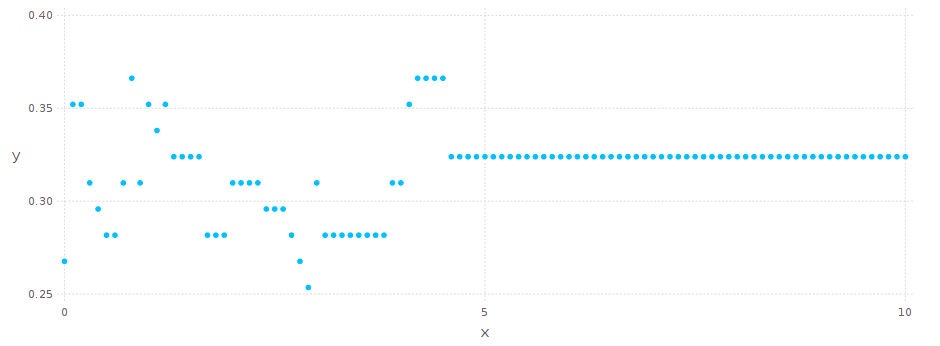
\includegraphics[width=400pt]{6_1_c.png}

So different values of $C$ can improve the accuracy of classification, but it
stays in the same order of magnitude.

But I don't understand, why the graph is so ``wobbly''.

\subsection{Teil d}

Classifying versicolor is hard, because they are very far from linearly
separable.

\subsection{Teil e}

\begin{lstlisting}
  kpoly(a,b,p,c) = (dot(a, b) + c)^p
\end{lstlisting}

\subsection{Teil f}

In ``svmtrain'' replace ``K = X * X''' with
\begin{lstlisting}
  K  = kernelmat(k, X, X)
\end{lstlisting}
and define ``svmpredictraw'' as
\begin{lstlisting}
  svmpredictraw(svm, X) = begin
    kernelmat(svm.k, X, svm.Xtrain) * diagm(svm.ytrain) * svm.alpha + svm.b
  end
\end{lstlisting}

\subsection{Teil g}

The Gaussian kernel function improved the classifier by an order of magnitude in
the worst case. Through manual testing I picked a bandwith of $4$, that
minimized the test errors. The updated errors are
\begin{tabular}{c|c}
  & Error\\\hline
  setosa & 0 \\\hline
  versicolor & 0.028 \\\hline
  virginica & 0.028
\end{tabular}
Increasing or decreasing $C$ resulted in an increase of the test error in all
cases.

\subsection{Teil h}

Polynomial kernels performed well, too. I got the best results with an ``offset''
of $3$ and an exponent of $2$.
\begin{tabular}{c|c}
  & Error\\\hline
  setosa & 0 \\\hline
  versicolor & 0.05 \\\hline
  virginica & 0.042
\end{tabular}
Increasing the exponent changed the errors only very little, while increasing
the ``offset'' increased the classification error of the ``versicolor'' iris to
$0.17$.

\subsection{Teil i}

\begin{lstlisting}
  k(a,b) = kgauss(a, b, 3)
  data = array(iris[:, 1:4])
  types = array(iris[:, 5])
  xs = 1:size(X, 1)
  setosa = filter(x -> types[x] == classes[1], xs)
  versicolor = filter(x -> types[x] == classes[2], xs)
  virginica = filter(x -> types[x] == classes[3], xs)

  X = [data[setosa, 1:4], data[versicolor, 1:4], data[virginica, 1:4]]

  K = kernelmat(k, X, X)
  imagesc(K)
\end{lstlisting}

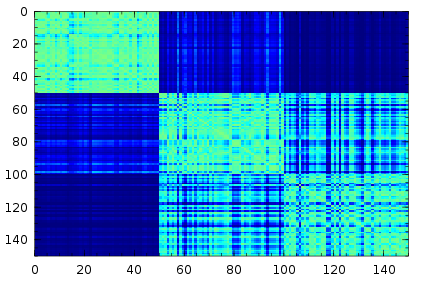
\includegraphics[width=300pt]{6_1_i.png}

The color of the cell $(x_{1}, x_{2})$ tells us the value of $k(x_{1}, x_{2})$,
whereas dark blue is close to $0$ and light blue is close to $1$. So in the
optimal case we would see 3 light blue squares on the diagonal on a dark blue
background. The dark blue rectangle tells us, that setosa are very dissimilar to
the rest, while the other two are harder to tell apart.

Increasing the bandwidth makes cells, that are even a little bit light blue,
lighter. So it rates things as more similar as it would with a lower bandwidth.

\section{Aufgabe 2}

\subsection{Teil a}

\begin{align*}
  \Phi(a)^{T}\Phi(b) & = (a_{1}^{2}, a_{2}^{2}, \sqrt{2}a_{1}a_{2}, \sqrt{2}a_{1}, \sqrt{2}a_{2}, 1)(b_{1}^{2}, b_{2}^{2}, \sqrt{2}b_{1}b_{2}, \sqrt{2}b_{1}, \sqrt{2}b_{2}, 1)^{T}\\
                     & = a_{1}^{2}b_{1}^{2} + a_{2}^{2}b_{2}^{2} + 2a_{1}b_{1}a_{2}b_{2} + 2 a_{1}b_{1} + 2 a_{2}b_{2} + 1\\
                     & = (a_{1}b_{1} + a_{2}b_{2} + 1)^{2}\\
                     & = (a^{T}b + 1)^{2}\\
                     & = k(a, b)
\end{align*}

\subsection{Teil b}

I will solve this by plugging values into the results of part c.

The feature space is of dimension
\begin{equation}
  \binom{2 + 3}{3} = \frac{5!}{3! \cdot 2!} = 10
\end{equation}

The feature map $\Phi$ is given by
\begin{equation}
  \Phi(a) = \begin{bmatrix}
    1\\
    \sqrt{3} a_{2}\\
    \sqrt{3} a_{2}^{2}\\
    a_{2}^{3}\\
    \sqrt{3} a_{1}\\
    \sqrt{6} a_{1} a_{2}\\
    \sqrt{3} a_{1} a_{2}^{2}\\
    \sqrt{3} a_{1}^{2}\\
    \sqrt{3} a_{1}^{2} a_{2}\\
    a_{1}^{3}
  \end{bmatrix}
\end{equation}

The feature map was generated by the following emacs-lisp program (which took
significantly longer to write than working out the functions by hand, but the
experience was worth it either way).
\lstset{language=Lisp}
\begin{lstlisting}
;;; Helper functions

(defun integer? (n)
  (= (floor n) n))

(defun factorial (n)
  (if (eq n 0)
      1
    (* n (factorial (- n 1)))))

(defun ncr (n ks)
  "n choose k - multinomial"
  (/ (factorial n) (-reduce #'* (-map #'factorial ks))))

(defun all-numbers? (nums)
  (cl-loop for n in nums always (numberp n)))

(defun one? (num)
  (and (numberp num) (= num 1)))

(defun monomials (n p)
  "Returns a list of all tuples of length N of positive numbers
  such that the numbers sum to P"
  (cond
   ((= n 1) (list (list p)))
   ((= n 0) '())
   (:else (cl-loop for i from 0 to p
                   nconc (cl-loop for j in (monomials (- n 1) (- p i))
                                  collect (cons i j))))))

;;; Functions to simplify the expressions

(defun simplify-sqrt (arg)
  (if (and (numberp arg) (integer? (sqrt arg)))
      (round (sqrt arg))
    `(sqrt ,arg)))

(defun simplify-binom (n &rest ks)
  (if (and (numberp n) (all-numbers? ks))
      (ncr n ks)
    `(binom ,n ,@ks)))

(defun simplify-+ (&rest nums)
  (if (all-numbers? nums)
      (apply #'+ nums)
    `(+ ,@nums)))

(defun simplify-* (&rest nums)
  (if (all-numbers? nums)
      (apply #'* nums)
    (let ((nums (-reject #'one? nums)))
      (if (one? (length nums))
          (car nums)
        `(* ,@nums)))))

(defun simplify-^ (base exponent)
  (cond
   ((and (numberp base) (numberp exponent))
    (expt base exponent))
   ((and (numberp exponent) (= exponent 0))
    1)
   ((and (numberp exponent) (= exponent 1))
    base)
   (:else
    `(^ ,base ,exponent))))

(defun simplify (expr)
  "Simplify an expression by evaluating sums and powers etc."
  (if (listp expr)
      (let* ((op (car expr))
             (args (-map #'simplify (cdr expr)))
             (fn (case op
                   ('sqrt #'simplify-sqrt)
                   ('binom #'simplify-binom)
                   ('+ #'simplify-+)
                   ('* #'simplify-*)
                   ('^ #'simplify-^))))
        (apply fn args))
    expr))

;;; Serialize to LaTeX

(defun to-latex-sqrt (n)
  (format "\\sqrt{%s}" n))

(defun to-latex-binom (n &rest ks)
  (format "\\binom{%s}{%s}" n (s-join ", \dots, " ks)))

(defun to-latex-+ (&rest nums)
  (s-join " + " nums))

(defun to-latex-* (&rest nums)
  (s-join " " nums))

(defun to-latex-^ (base exponent)
  (format "%s^{%s}" base exponent))

(defun to-latex (expr)
  (cond
   ((listp expr)
    (let* ((op (car expr))
           (args (-map #'to-latex (cdr expr)))
           (fn (case op
                 ('sqrt #'to-latex-sqrt)
                 ('binom #'to-latex-binom)
                 ('+ #'to-latex-+)
                 ('* #'to-latex-*)
                 ('^ #'to-latex-^))))
      (apply fn args)))
   ((numberp expr)
    (number-to-string expr))
   (:else
    expr)))

;;; Generate expressions

(defun fn-expressions (n p)
  "Generates expressions for the component functions of the
feature map of the form, that was worked out in part c.

- N is the dimensionality of the attribute space
- P is the degree of the polynomial kernel function"
  (cl-loop for m in (monomials (+ n 1) p)
           collect `(*
                     (sqrt (binom ,p ,@m))
                     (*
                      (^ "a_{1}" ,(car m))
                      (^ "a_{2}" ,(cadr m))
                      (^ 1 ,(caddr m))))))

(defun feature-function (n p)
  "Generate the feature function, simplify it and convert it to
latex"
  (let* ((fns (fn-expressions n p))
         (simplified (-map #'simplify fns)))
    (s-join "\\\\\n"
            (-map #'to-latex simplified))))

;; Print the feature function
(message "%s" (feature-function 2 3))
\end{lstlisting}

\subsection{Teil c}

\begin{align*}
  k(a, b) & = (a^{T}b + 1)^{p}\\
          & = \left( 1 + \sum_{i = 1}^{n} a_{i}b_{i} \right)^{p}\\
          & = \sum_{k_{1} + \dots + k_{n} + k_{n + 1} = p} \binom{p}{k_{1}, \dots, k_{n + 1}} \left( \prod_{i = 1}^{n} (a_{i}b_{i})^{k_{i}} \right) \cdot 1^{k_{n + 1}} \quad \textit{multinomial theorem}\\
          & = \sum_{k_{1} + \dots + k_{n} + k_{n + 1} = p} \binom{p}{k_{1}, \dots, k_{n + 1}} \prod_{i = 1}^{n} (a_{i}b_{i})^{k_{i}}\\
          & = \sum_{k_{1} + \dots + k_{n} + k_{n + 1} = p} \binom{p}{k_{1}, \dots, k_{n + 1}} \prod_{i = 1}^{n} a_{i}^{k_{i}}b_{i}^{k_{i}}\\
          & = \sum_{k_{1} + \dots + k_{n} + k_{n + 1} = p} \left( \sqrt{\binom{p}{k_{1}, \dots, k_{n + 1}}} \prod_{i = 1}^{n} a_{i}^{k_{i}} \right) \left( \sqrt{\binom{p}{k_{1}, \dots, k_{n + 1}}} \prod_{i = 1}^{n} b_{i}^{k_{i}} \right)\\
          & = \Phi(a)^{T}\Phi(b)
\end{align*}
So the feature mapping $\Phi$ is a function
$\mathbb{R}^{n} \mapsto \mathbb{R}^{m}$, where $m$ is the number of ways to pick
$0 \le k_{1}, \dots, k_{n + 1} \le p$, such that
$\sum_{i = 1}^{n + 1} k_{i} = p$ respectively the number of monomials up to
degree $p$
\begin{equation}
  m = \binom{p + (n + 1) - 1}{p} = \binom{p + n}{p}
\end{equation}
The dimensionality of the feature space is also $m$.

Let $K$ be a sequence of tuples $(k_{1}, \dots, k_{n + 1})$ of positive integers
$k_{i}$, such that $\sum_{i = 1}^{n + 1}K_{j, i} = p \quad \forall j = 1..m$. Then
the $j$th component of the feature mapping $\Phi$ is given by
\begin{equation}
  \Phi_{j}(a) = \sqrt{\binom{p}{K_{j}}} \prod_{i = 1}^{n} a_{i}^{K_{j, i}}
\end{equation}
modulo order of components.

\end{document}